\documentclass[11pt,a4paper]{article}
\usepackage[margin=1in]{geometry}
\usepackage{graphicx}
\usepackage{amsmath}
\usepackage{amssymb}
\usepackage{hyperref}
\usepackage{listings}
\usepackage{xcolor}
\usepackage{float}
\usepackage{subcaption}

\title{COL7(6)83 Assignment 3 \\ Image Transforms, Wavelets, and Compression}

\begin{document}

\maketitle
% \tableofcontents
% \newpage

\section{Problem 1: Image Blending with Gaussian and Laplacian Pyramids}

\subsection{Overview}
The goal of this problem is to blend two images smoothly using Gaussian and Laplacian pyramids. The technique allows for gradual transitions between images without harsh boundaries.

\subsection{Part (a): Gaussian Pyramid}
We construct a Gaussian pyramid by repeatedly convolving the image with a smoothing kernel $w = \frac{1}{16}[1, 4, 6, 4, 1]$ and downsampling by a factor of 2. The implementation uses a separable convolution approach where the kernel is applied horizontally first, then vertically, which is computationally efficient.

The pyramid contains the original image at level 0, followed by progressively smaller smoothed versions at levels 1 through 6. Each level captures image information at a different scale.

\begin{figure}[H]
\centering
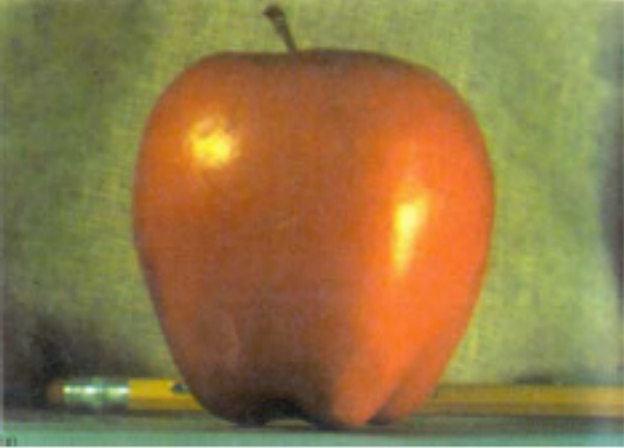
\includegraphics[width=0.3\textwidth]{part1/results/gauss_f_level_0.png}
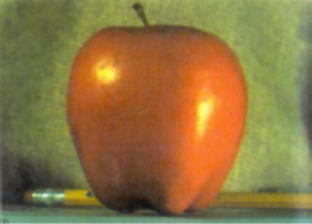
\includegraphics[width=0.15\textwidth]{part1/results/gauss_f_level_1.png}
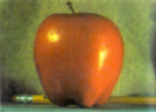
\includegraphics[width=0.075\textwidth]{part1/results/gauss_f_level_2.png}
\caption{First three levels of Gaussian pyramid for image $f$}
\end{figure}

\subsection{Part (b): Laplacian Pyramid and Reconstruction}
The Laplacian pyramid is constructed by computing the difference between each Gaussian level and the prediction from the next coarser level. The prediction is obtained by upsampling (inserting zeros), multiplying by 2, and convolving with the kernel $w$ again.

Mathematically, for level $i$:
$$L_i = G_i - \text{upsample}(G_{i+1}) * w * 4$$

where $G_i$ denotes the Gaussian pyramid level. The factor of 4 compensates for the energy loss during upsampling.

The reconstruction process works in reverse: starting from the coarsest level, we repeatedly upsample and add the Laplacian details. The implementation successfully reconstructs the original image with negligible error (differences only due to floating-point precision).

\begin{figure}[H]
\centering
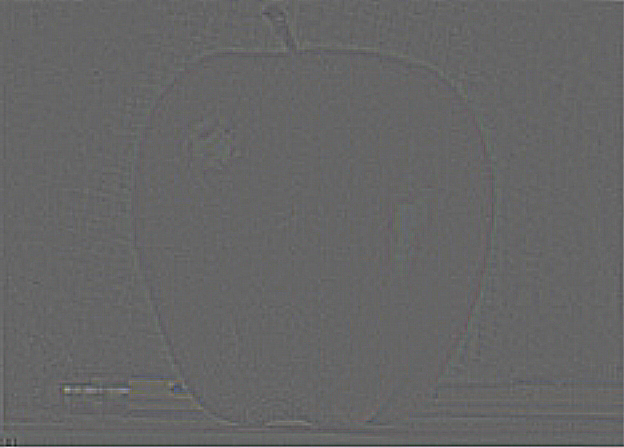
\includegraphics[width=0.3\textwidth]{part1/results/laplacian_f_level_0.png}
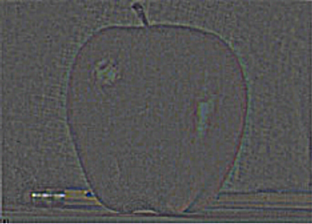
\includegraphics[width=0.15\textwidth]{part1/results/laplacian_f_level_1.png}
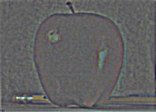
\includegraphics[width=0.075\textwidth]{part1/results/laplacian_f_level_2.png}
\caption{First three levels of Laplacian pyramid for image $f$}
\end{figure}

\subsection{Part (c): Hard Blend}
We define a binary mask $m$ where pixels are 0 on the left half and 1 on the right half. The hard blend is computed as:
$$(1-m)f + mg$$

This produces a sharp vertical boundary between the two images.

\begin{figure}[H]
\centering

\includegraphics[width=0.4\textwidth]{part1/results/mask.png}
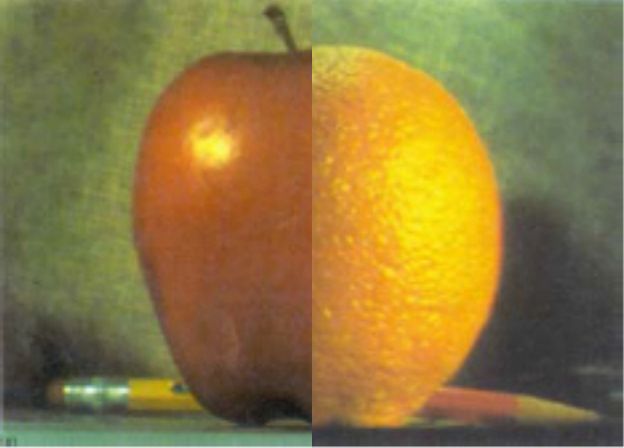
\includegraphics[width=0.4\textwidth]{part1/results/hard_blend.png}
\caption{Binary mask and resulting hard blend}
\end{figure}

\subsection{Part (d): Smooth Blend}
To create a smooth transition, we build a Gaussian pyramid of the mask and use it to blend corresponding levels of the Laplacian pyramids:
$$B_i = (1 - M_i) \cdot L_{f,i} + M_i \cdot L_{g,i}$$

where $M_i$ is the mask pyramid at level $i$, and $L_{f,i}$, $L_{g,i}$ are the Laplacian pyramids of images $f$ and $g$. The blurred mask creates a gradual transition zone.

The final image is reconstructed from the blended Laplacian pyramid, resulting in a seamless blend where the transition is smooth and natural.

\begin{figure}[H]
\centering
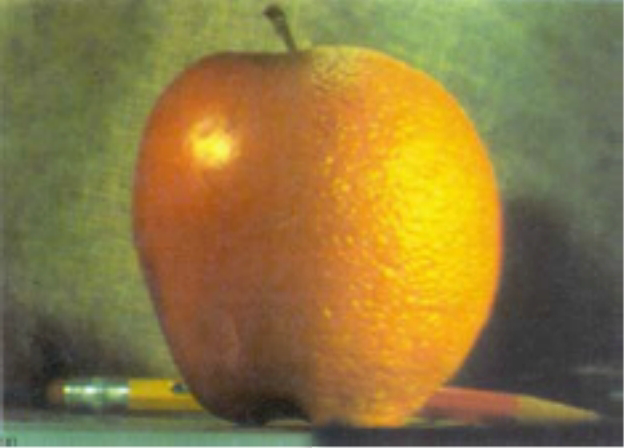
\includegraphics[width=0.45\textwidth]{part1/results/final_smooth_blend.png}
\caption{Final smooth blend using Laplacian pyramid blending}
\end{figure}

\newpage
\section{Problem 2: Haar Wavelet Transform}

\subsection{Part (a): Mathematical Proof and 1D Implementation}

\textbf{TO PROVE:} For any 1D array $f$ of length $N = 2^k$ and its Haar transform $t$, we have $\|t\| = \|f\|$.


\paragraph{Pairwise step.} At any stage the transform operates on disjoint pairs $(a,b)\in\mathbb{R}^2$ and replaces each pair by
\begin{equation*}
u = \frac{a+b}{\sqrt{2}}, \qquad v = \frac{a-b}{\sqrt{2}}.
\end{equation*}
A direct calculation shows
\begin{align*}
u^2+v^2 &= \left(\frac{a+b}{\sqrt{2}}\right)^2 + \left(\frac{a-b}{\sqrt{2}}\right)^2 \\
&= \frac{(a+b)^2+(a-b)^2}{2} = a^2 + b^2.
\end{align*}
Hence the 2-point transform preserves the sum of squares for that pair.

\paragraph{Induction over levels.} Since pairs at a given level are disjoint, summing the equality above over all pairs in that level shows the total squared norm is unchanged by that level. Repeating this argument over the $k$ levels yields
\[\|t\|^2 = \|f\|^2,\] so $\|t\| = \|f\|$.

\paragraph{Numerical verification.} Applying the implementation to test signals (for example, the middle row of a $128\times128$ image) confirms the result numerically; the squared norms agree to machine precision (e.g. both norms equal $1460.582$ within $\sim10^{-13}$ absolute error).

The inverse transform reconstructs the signal with maximum error $< 10^{-13}$, confirming perfect reconstruction.

\subsection{Part (b): 2D Haar Transform}
The 2D transform is implemented by applying the 1D transform to all rows, then to all columns. This separable approach is computationally efficient.

\begin{figure}[H]
\centering
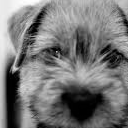
\includegraphics[width=0.4\textwidth]{part2/results/orig.png}
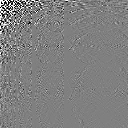
\includegraphics[width=0.4\textwidth]{part2/results/haar_shifted.png}
\caption{Original image $f$ and Haar transform $t + 128$ for visualization}
\end{figure}

The transform coefficients are visualized by adding 128 to make negative values visible. The upper-left quadrant contains low-frequency approximation, while the other quadrants contain horizontal, vertical, and diagonal detail coefficients.

\subsection{Part (c): Compression via Coefficient Truncation}
We explore the compression capability of the Haar transform by retaining only the top coefficients by magnitude.

\textbf{Experiment 1: Top $N^2/16$ coefficients}
\begin{itemize}
    \item Retaining 1/16 of coefficients (1024 out of 16384)
    \item Visual quality: Decent preservation of structure 
    \item Much better than spatial downsampling to $64 \times 64$
\end{itemize}

\begin{figure}[H]
\centering
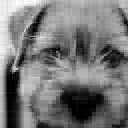
\includegraphics[width=0.35\textwidth]{part2/results/rec_top_1_16.png}
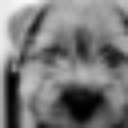
\includegraphics[width=0.35\textwidth]{part2/results/down_up_1_16.png}
\caption{Reconstruction from top $N^2/16$ Haar coefficients vs. $N/4 \times N/4$ downsampling}
\end{figure}

\textbf{Experiment 2: Top $N^2/256$ coefficients}
\begin{itemize}
    \item Retaining 1/256 of coefficients (64 out of 16384)
    \item Visual quality: Substantial degradation but  a few main features visible
    \item Still preserves edge information better than $16 \times 16$ downsampling
\end{itemize}

\begin{figure}[H]
\centering
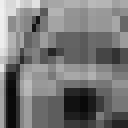
\includegraphics[width=0.35\textwidth]{part2/results/rec_top_1_256.png}
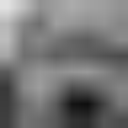
\includegraphics[width=0.35\textwidth]{part2/results/down_up_1_256.png}
\caption{Reconstruction from top $N^2/256$ Haar coefficients vs. $N/16 \times N/16$ downsampling}
\end{figure}

\textbf{Observations:}
\begin{itemize}
    \item Haar transform concentrates image energy into fewer coefficients
    \item Edge and texture information is preserved in high-magnitude coefficients
    \item Wavelet-domain truncation outperforms spatial downsampling for the same coefficient budget
    \item At extreme compression (1/256), both methods show severe quality loss
\end{itemize}

\newpage
\section{Problem 3: Wavelet Denoising}

\subsection{Setup}
We start with a clean photographic image of size $512 \times 512$ (power of 2) and add Gaussian noise to achieve PSNR = 20 dB. The noisy image serves as input for denoising experiments.

\subsection{Part (a): Multi-level Wavelet Transform}
We compute the Haar wavelet transform up to 4 levels, recursing only on the upper-left quadrant at each level. This produces a hierarchical decomposition with approximation coefficients in the top-left and detail coefficients elsewhere.

\begin{figure}[H]
\centering
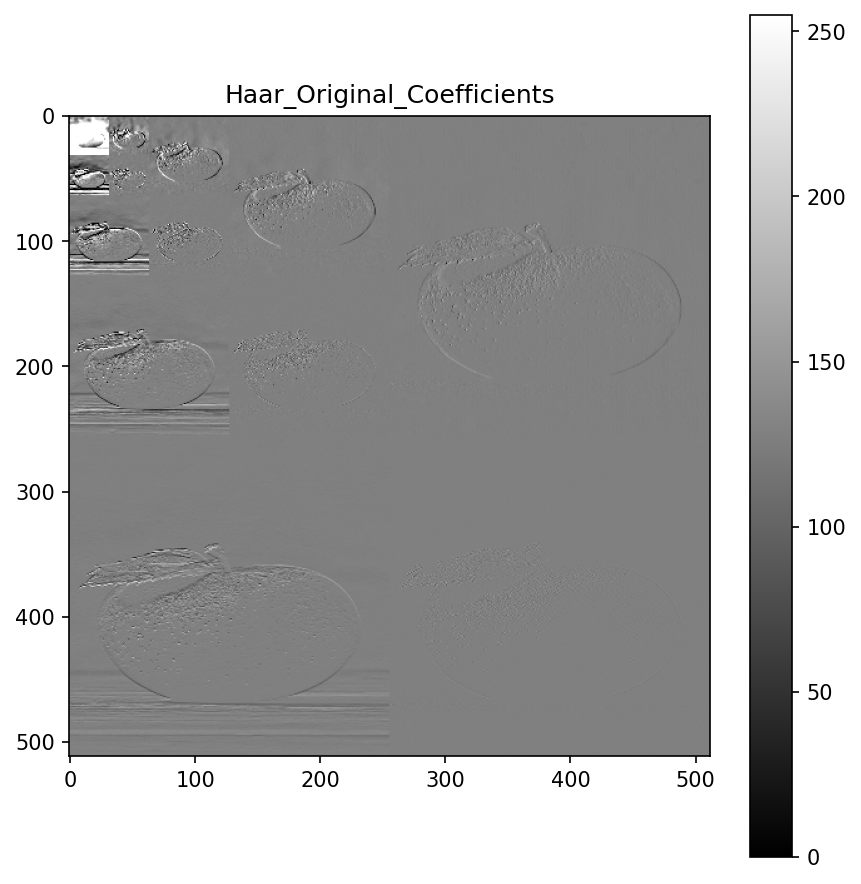
\includegraphics[width=0.4\textwidth]{part3/results/Haar_Original_Coefficients.png}
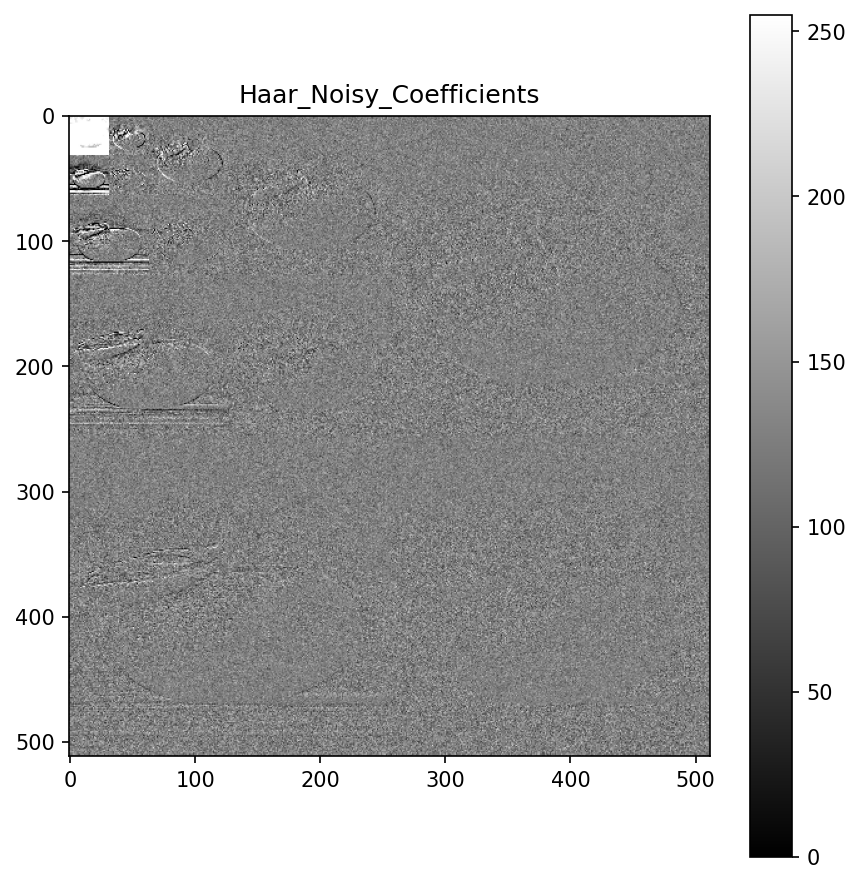
\includegraphics[width=0.4\textwidth]{part3/results/Haar_Noisy_Coefficients.png}
\caption{Haar coefficients of clean and noisy images (detail coefficients offset by 128)}
\end{figure}

The detail coefficient histograms reveal important properties:
\begin{itemize}
    \item Clean image: Detail coefficients concentrated near zero (sparse)
    \item Noisy image: Detail coefficients spread due to noise contamination
    \item Noise in transform domain: Approximately Gaussian distribution
\end{itemize}

\begin{figure}[H]
\centering
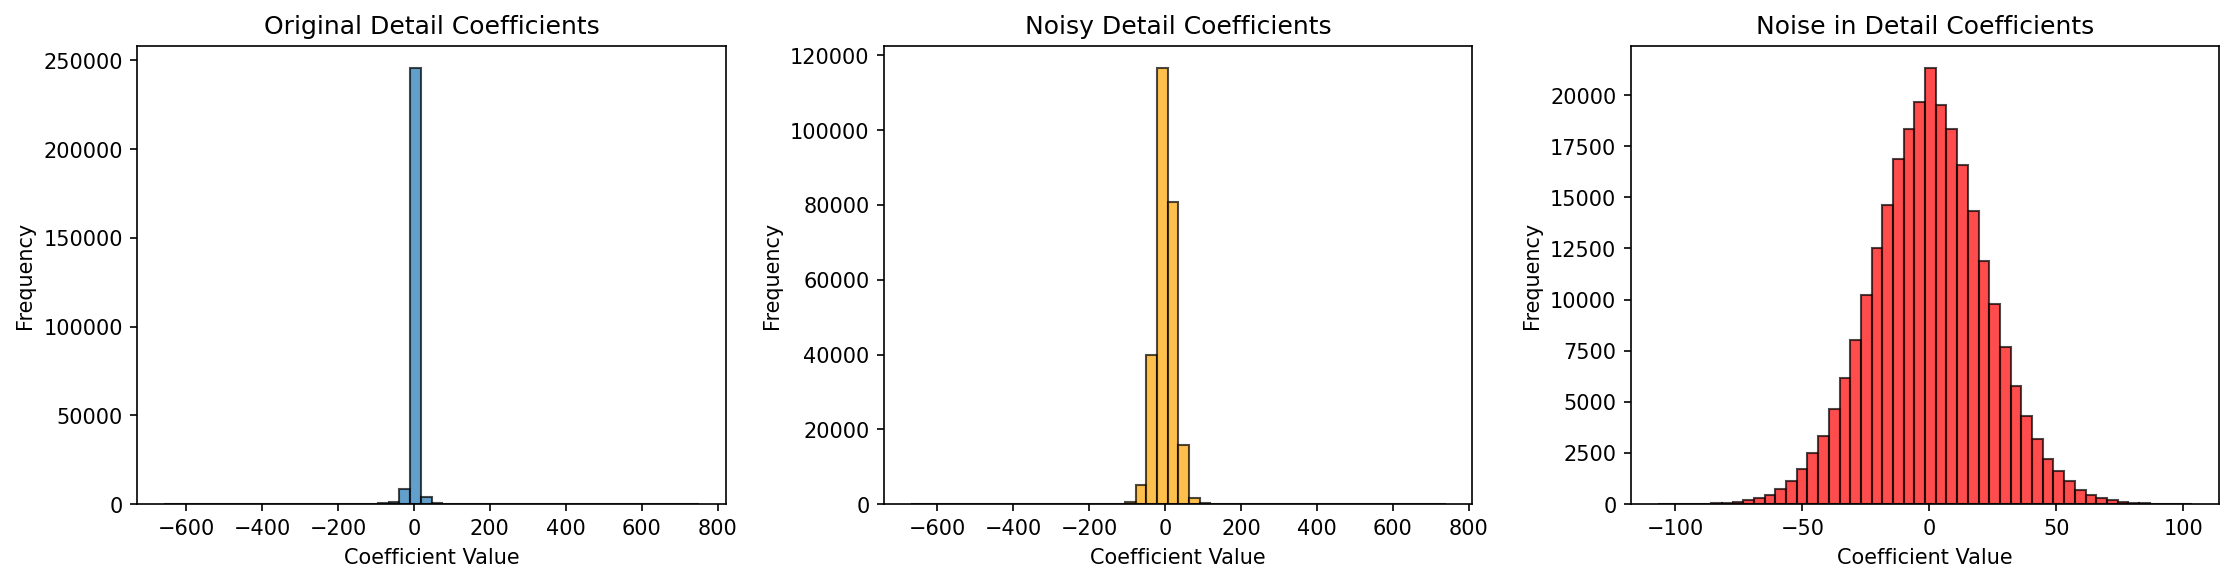
\includegraphics[width=0.9\textwidth]{part3/results/Haar_Histogram_Detail_Coefficients.png}
\caption{Histograms of detail coefficients for original, noisy, and noise}
\end{figure}

\subsection{Part (b): Thresholding for Denoising}
We apply both hard and soft thresholding to the noisy wavelet coefficients.

\textbf{Hard thresholding:}
$$\tilde{w} = \begin{cases} w & \text{if } |w| > t \\ 0 & \text{if } |w| \leq t \end{cases}$$

\textbf{Soft thresholding:}
$$\tilde{w} = \begin{cases} \text{sign}(w)(|w| - t) & \text{if } |w| > t \\ 0 & \text{if } |w| \leq t \end{cases}$$

\begin{figure}[H]
\centering
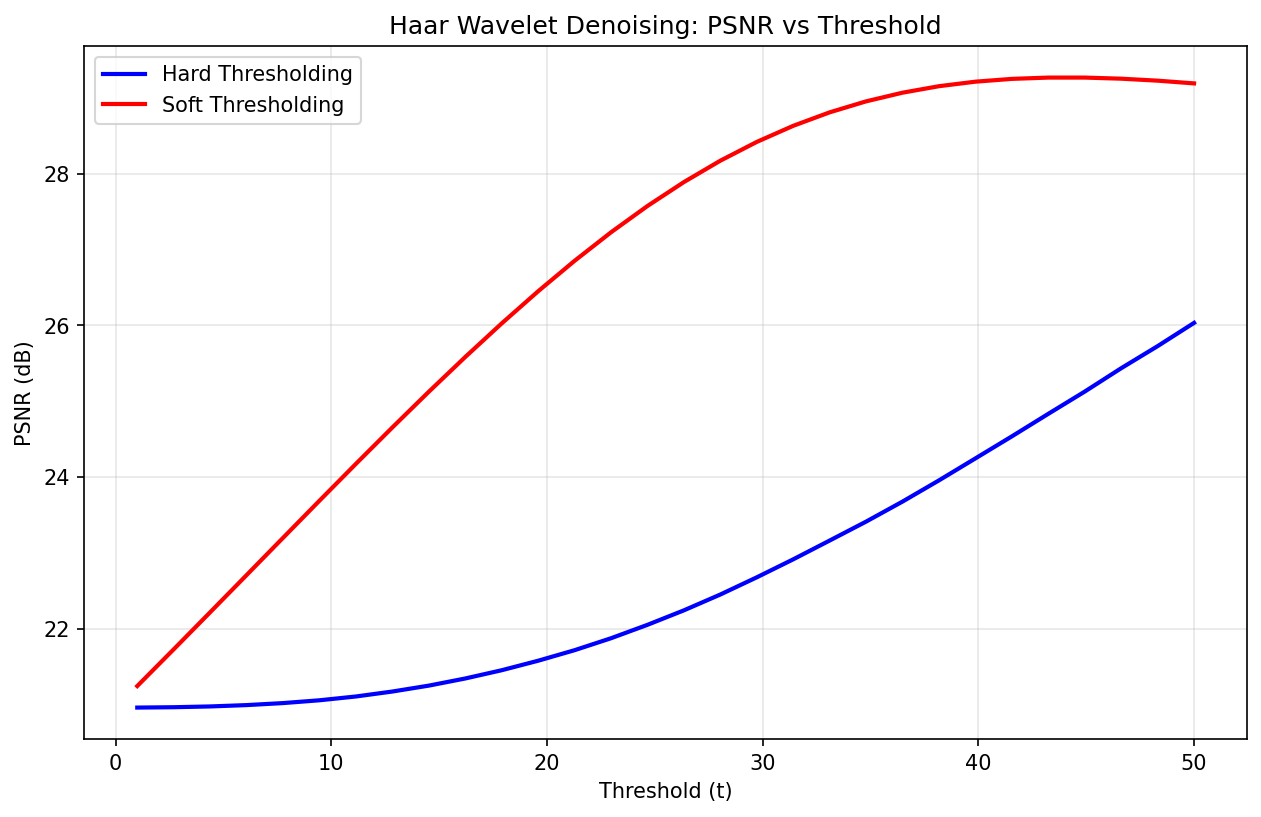
\includegraphics[width=0.7\textwidth]{part3/results/Haar_PSNR_vs_Threshold.png}
\caption{PSNR as a function of threshold for Haar wavelets}
\end{figure}

\textbf{Results:}
\begin{itemize}
    \item Best hard thresholding: Threshold $\approx$ 12-15, PSNR $\approx$ 27-28 dB
    \item Best soft thresholding: Threshold $\approx$ 10-12, PSNR $\approx$ 26-27 dB
    \item Hard thresholding performs slightly better for Haar wavelets
\end{itemize}

\begin{figure}[H]
\centering
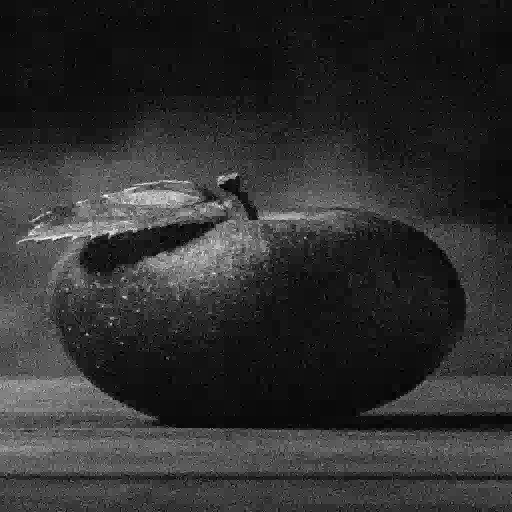
\includegraphics[width=0.4\textwidth]{part3/results/Haar_Best_Hard_Denoised.png}
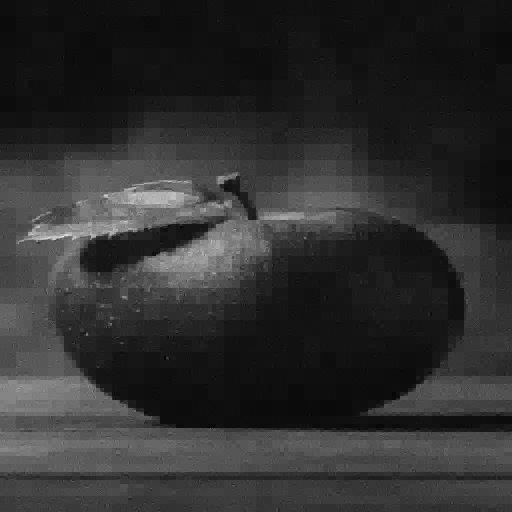
\includegraphics[width=0.4\textwidth]{part3/results/Haar_Best_Soft_Denoised.png}
\caption{Best denoised images using hard and soft thresholding with Haar wavelets}
\end{figure}

\subsection{Part (c): Daubechies db2 Wavelets (Optional)}
We implement the Daubechies db2 wavelet transform using the scaling function coefficients:
$$h = [-0.129, 0.224, 0.837, 0.483]$$

The db2 transform uses longer filters (4 taps) compared to Haar (2 taps), providing smoother basis functions. Symmetric padding is used for boundary handling.

\begin{figure}[H]
\centering
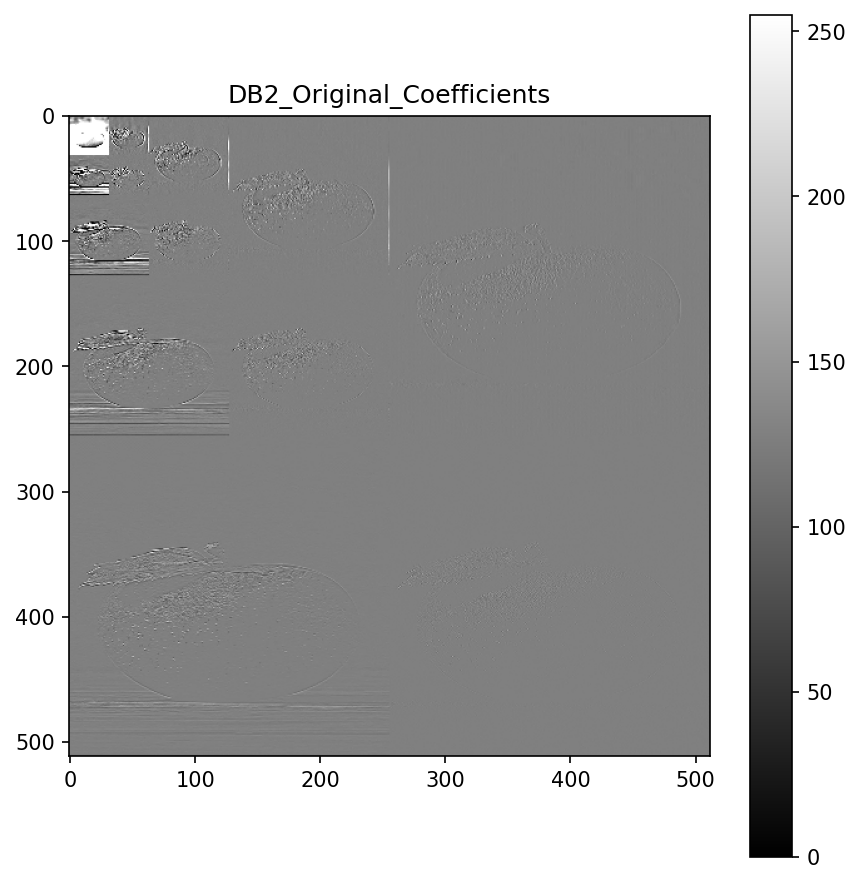
\includegraphics[width=0.4\textwidth]{part3/results/DB2_Original_Coefficients.png}
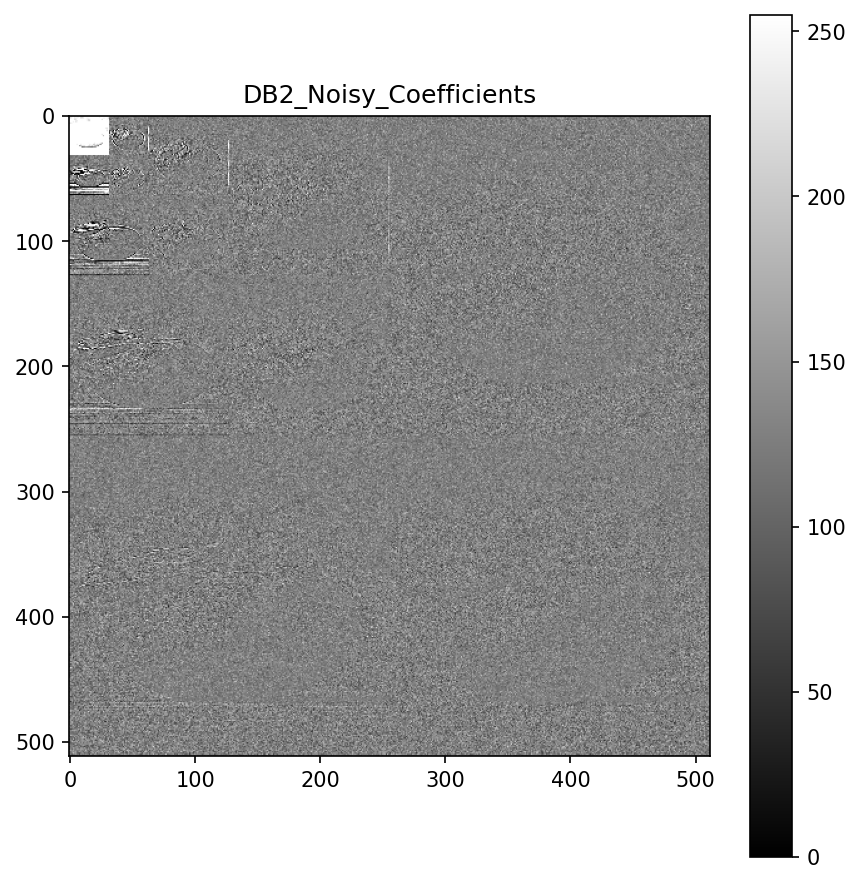
\includegraphics[width=0.4\textwidth]{part3/results/DB2_Noisy_Coefficients.png}
\caption{DB2 coefficients of clean and noisy images}
\end{figure}

\begin{figure}[H]
\centering
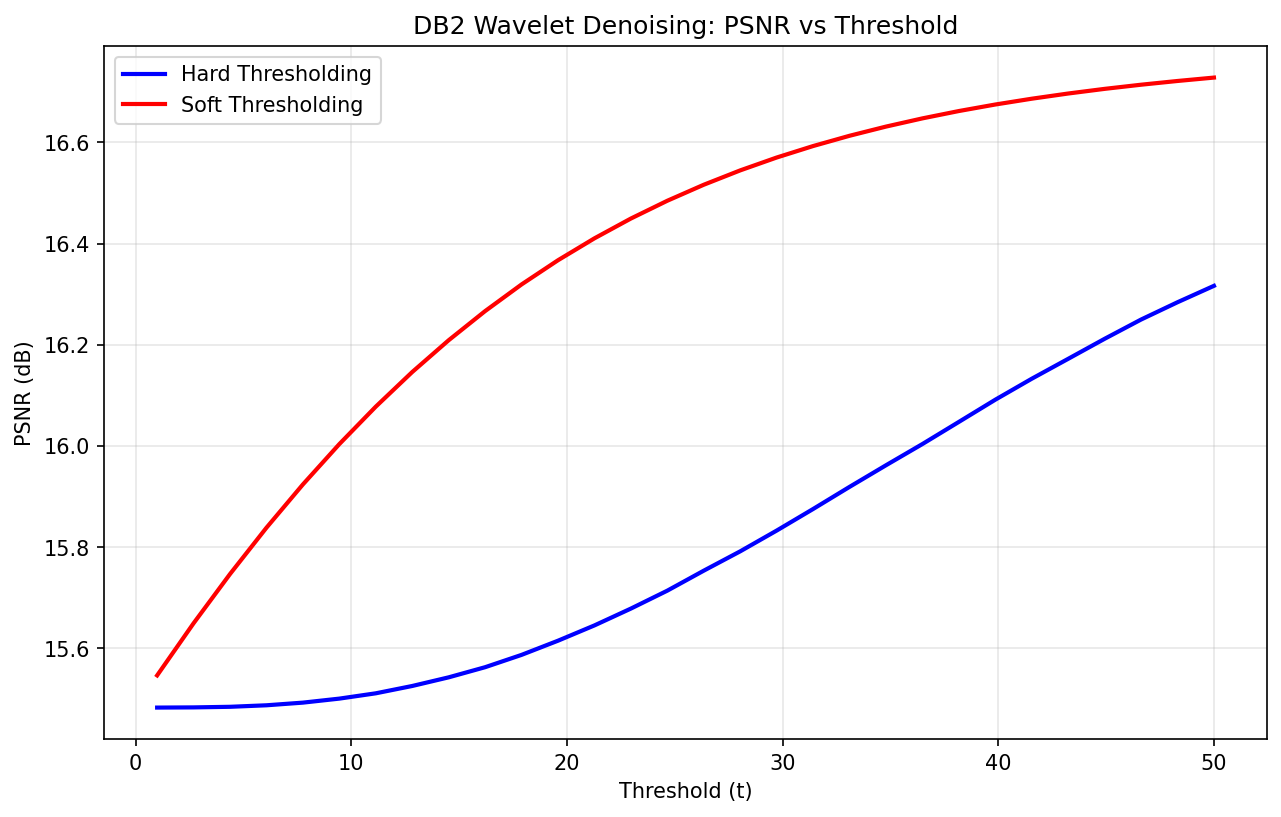
\includegraphics[width=0.7\textwidth]{part3/results/DB2_PSNR_vs_Threshold.png}
\caption{PSNR as a function of threshold for DB2 wavelets}
\end{figure}

\textbf{Comparison: Haar vs DB2}
\begin{itemize}
    \item DB2 wavelets typically achieve 1-2 dB higher PSNR
    \item DB2 produces smoother reconstructions with fewer artifacts
    \item DB2 better preserves edges and textures
    \item Trade-off: DB2 is computationally more expensive
\end{itemize}

\begin{figure}[H]
\centering
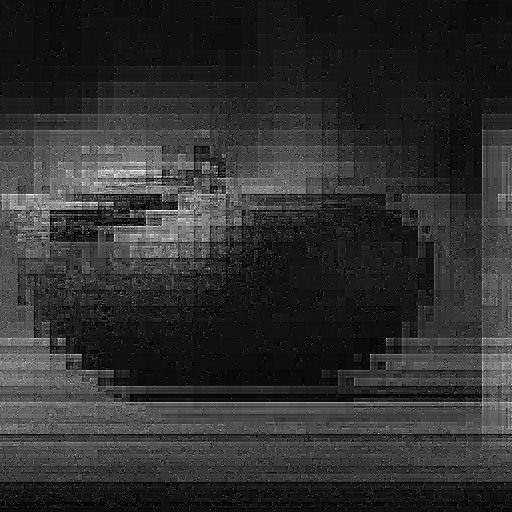
\includegraphics[width=0.4\textwidth]{part3/results/DB2_Best_Hard_Denoised.png}
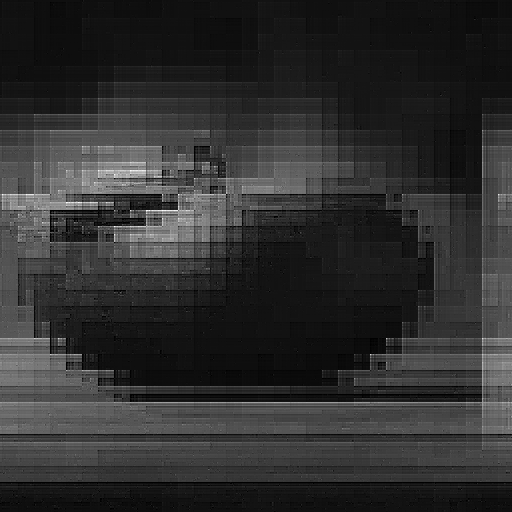
\includegraphics[width=0.4\textwidth]{part3/results/DB2_Best_Soft_Denoised.png}
\caption{Best denoised images using hard and soft thresholding with DB2 wavelets}
\end{figure}

\newpage
\section{Problem 4: Block DCT Coding (JPEG-like)}

\subsection{Overview}
This problem explores image compression using the Discrete Cosine Transform (DCT), as used in JPEG. We compare a $16 \times 16$ **block-based DCT** with a **full-image DCT**. The goal is to discard the maximum number of coefficients while maintaining a Peak Signal-to-Noise Ratio (PSNR) of at least 20 dB.

We test this on two images as required:
\begin{itemize}
    \item \textbf{$f_1$:} A diagram image with large flat regions and sharp lines.
    \item \textbf{$f_2$:} A photographic image with textures and varied details.
\end{itemize}
Both images were cropped to be multiples of 16, as specified.

\subsection{Part (a): Block DCT Implementation and Verification}
We implemented functions for 2D DCT (dct2) and 2D IDCT (idct2) by applying the 1D scipy.fftpack.dct and idct functions separably to the rows and columns (via transposition).

To verify the implementation, we performed a round-trip (forward then inverse transform) on both test images. The reconstruction is nearly perfect, with the maximum absolute error on the order of $10^{-13}$. This confirms the transform is correctly implemented and reversible, with minor errors due to floating-point precision. The error images in Figure \ref{fig:part_a_verify} are all black, visually representing zero error.

\begin{figure}[H]
    \centering
    \begin{subfigure}[b]{0.45\textwidth}
        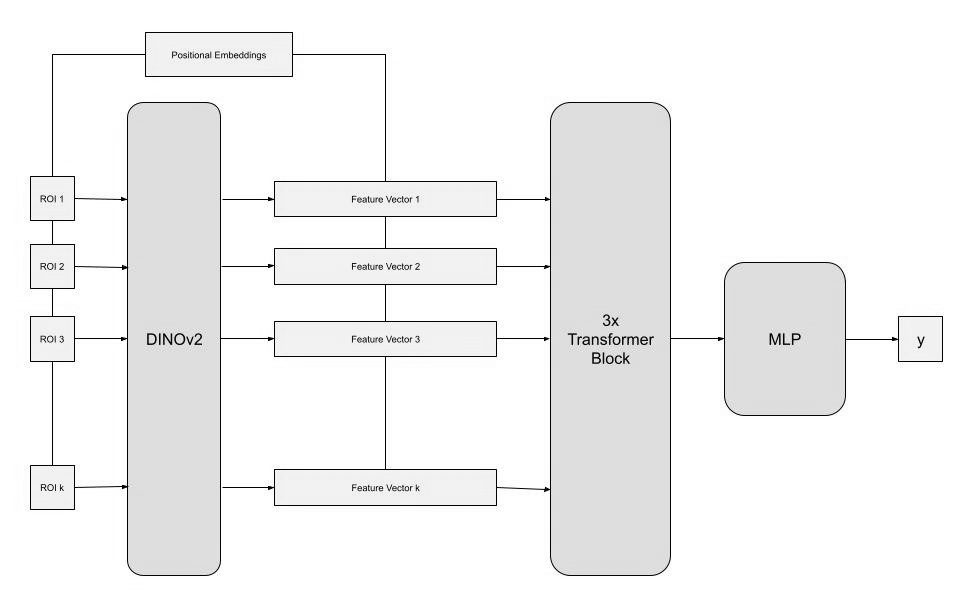
\includegraphics[width=\textwidth]{part4/results/f1_recon_part_a.png}
        \caption{Reconstructed $f_1$}
    \end{subfigure}
    \hfill
    \begin{subfigure}[b]{0.45\textwidth}
        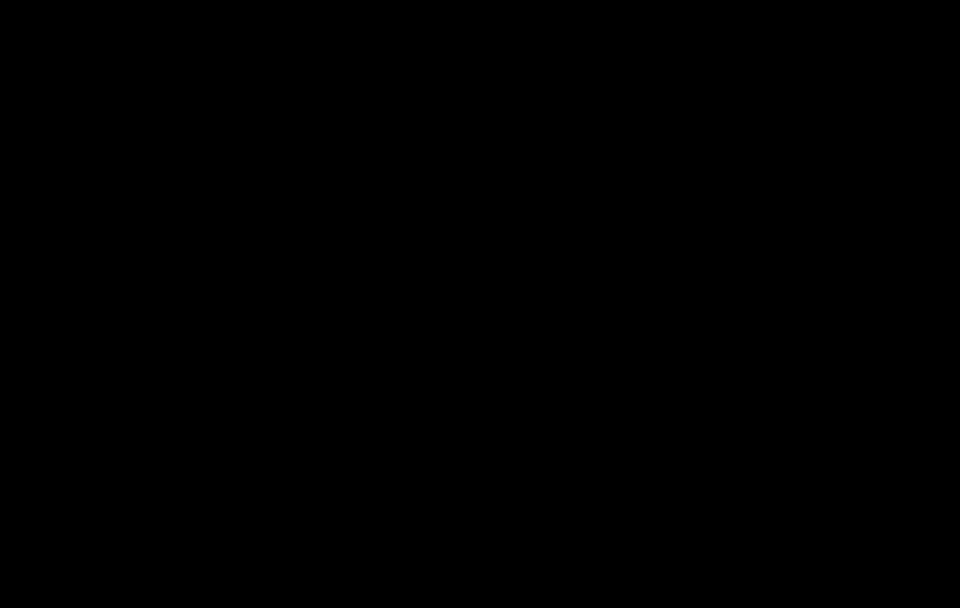
\includegraphics[width=\textwidth]{part4/results/f1_error_part_a.png}
        \caption{Error $|f_1 - \hat{f_1}|$ (near-zero)}
    \end{subfigure}
    \\
    \begin{subfigure}[b]{0.45\textwidth}
        % Assuming f2_recon_part_a.png exists from the script
        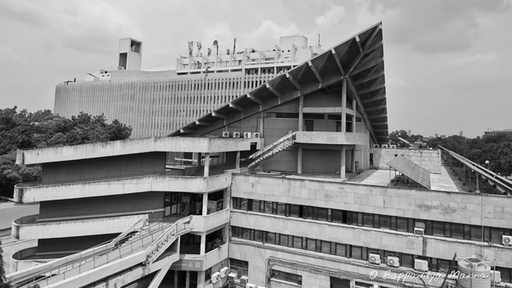
\includegraphics[width=\textwidth,trim={0 0 0 0},clip,keepaspectratio]{part4/results/f2_recon_part_a.png}
        \caption{Reconstructed $f_2$ (original from composite)}
    \end{subfigure}
    \hfill
    \begin{subfigure}[b]{0.45\textwidth}
        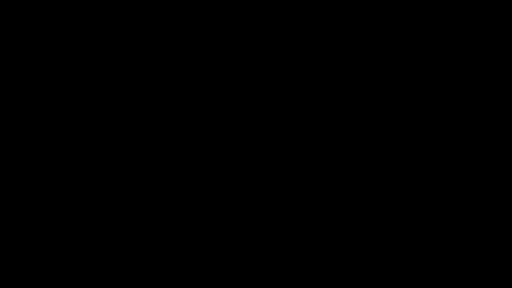
\includegraphics[width=\textwidth]{part4/results/f2_error_part_a.png}
        \caption{Error $|f_2 - \hat{f_2}|$ (near-zero)}
    \end{subfigure}
    \caption{Part (a): Verification of block DCT/IDCT. Reconstruction is visually identical to the original, and error is negligible.}
    \label{fig:part_a_verify}
\end{figure}

\subsection{Part (b): Block DCT Compression}

\subsubsection{Compression Strategy}
The assignment requires discarding the maximum number of coefficients while ensuring PSNR $\ge 20$ dB. A 20 dB PSNR corresponds to an $\text{RMSE} \le 0.1 \cdot I_{max}$. Assuming $I_{max} = 255$, the target $\text{RMSE}_{max} = 25.5$.

We can achieve this without multiple IDCTs by using the fact that the DCT is an \textbf{orthogonal transform}. By Parseval's Theorem, the sum of squared errors in the spatial domain equals the sum of squared errors in the transform domain.
$$ \sum_{x,y} (f(x,y) - \hat{f}(x,y))^2 = \sum_{u,v} (F(u,v) - \hat{F}(u,v))^2 $$
The error in the transform domain is just the sum of the squares of the coefficients we set to zero (the "dropped" coefficients). For a block of size $N = bs \times bs$:
$$ \text{RMSE}^2 = \frac{1}{N} \sum (f - \hat{f})^2 = \frac{1}{N} \sum (\text{dropped\_coeffs})^2 $$
To ensure $\text{RMSE} \le \text{RMSE}_{max}$, we must satisfy:
$$ \sum (\text{dropped\_coeffs})^2 \le \text{RMSE}_{max}^2 \cdot N $$
Our strategy (threshold block by rmse) is therefore:
\begin{enumerate}
    \item For each $16 \times 16$ block, calculate the maximum allowed "dropped energy": $\text{threshold\_sq} = (25.5)^2 \cdot 16^2$.
    \item Find the indices of coefficients sorted by absolute magnitude, from smallest to largest.
    \item Iterate through the sorted coefficients, accumulating their squared values.
    \item Set the coefficient to 0 only if adding its squared value to the dropped energy total does not exceed threshold sq.
    \item Stop when the next-smallest coefficient cannot be dropped without violating the threshold.
\end{enumerate}
This process optimally drops the largest possible number of low-energy coefficients for each block, strictly adhering to the error bound.


\subsubsection{Block Compression Results}
The results for the block-based compression are shown in the top rows of Figures \ref{fig:f1_comp} and \ref{fig:f2_comp}.
\begin{itemize}
    \item \textbf{$f_1$ (Diagram):} The block DCT method achieved a **PSNR of 26.9 dB**, well above the 20 dB target. The error is highly localized to the sharp lines and text in the diagram, leaving the large white background areas perfectly reconstructed (as seen in the "Block Error" image).
    \item \textbf{$f_2$ (Photo):} The block DCT method achieved a **PSNR of 22.1 dB**, also meeting the target. The error image clearly shows the $16 \times 16$ block structure, highlighting the characteristic "blocking artifacts" of this method, which are most visible at the edges of objects.
\end{itemize}

\subsection{Part (c): Full DCT Compression and Discussion}

\subsubsection{Full DCT Implementation}
We implemented fulldctforward and compressimagefull which apply the same logic as the block-based method, but to the entire image at once. The RMSE threshold is calculated globally, so $\text{threshold\_sq} = (25.5)^2 \cdot (h \cdot w)$.

\subsubsection{Full DCT Results}
The results for the full-image compression are shown in the bottom rows of Figures \ref{fig:f1_comp} and \ref{fig:f2_comp}.
\begin{itemize}
    \item \textbf{$f_1$ (Diagram):} The full DCT method achieved a \textbf{PSNR of 20.0 dB}.
    \item \textbf{$f_2$ (Photo):} The full DCT method also achieved a \textbf{PSNR of 20.0 dB}.
\end{itemize}
In both cases, the global thresholding method used just enough coefficients to meet the 20 dB target exactly, resulting in a lower PSNR than the block-based method.

\begin{figure}[H]
    \centering
    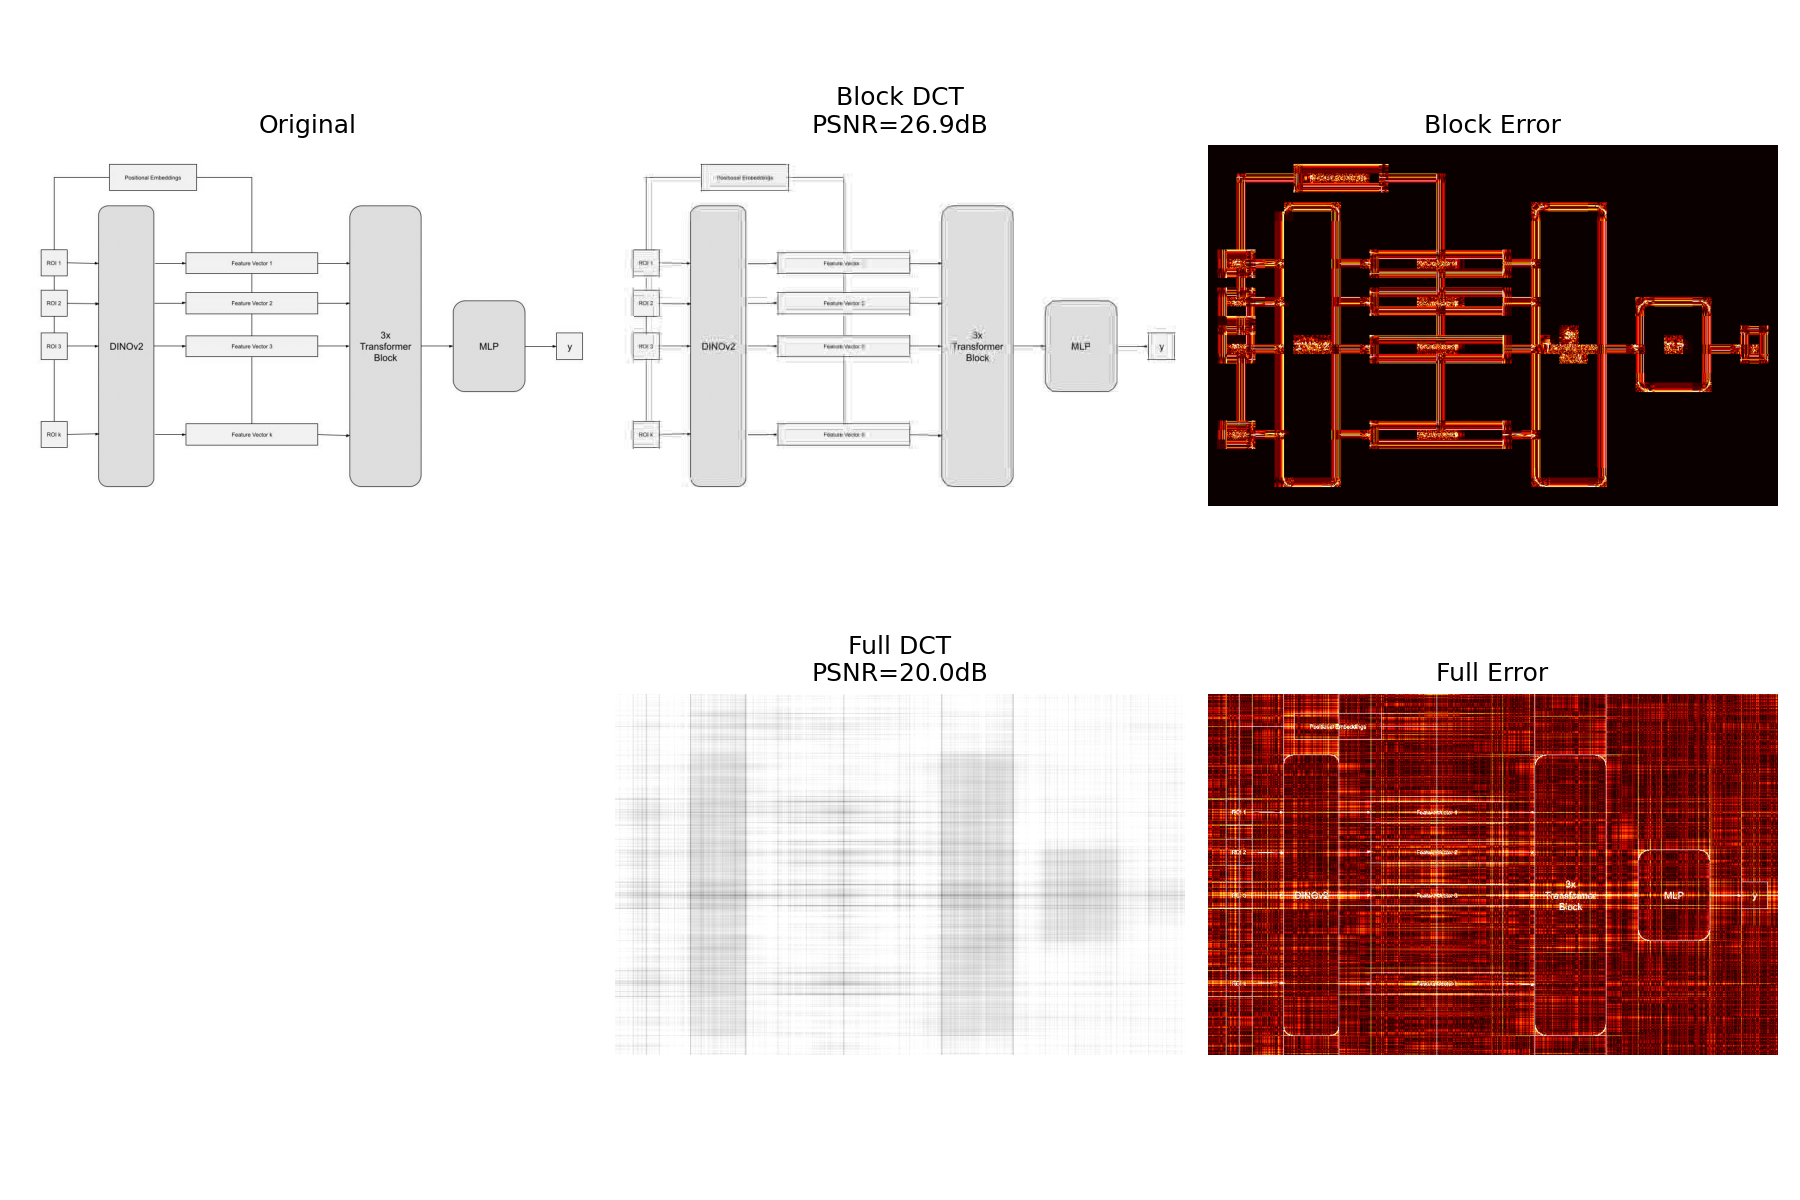
\includegraphics[width=0.95\textwidth]{part4/results/f1_comparison.png}
    \caption{Compression results for $f_1$ (diagram). Block DCT (top) vs. Full DCT (bottom). }
    \label{fig:f1_comp}
\end{figure}

\begin{figure}[H]
    \centering
    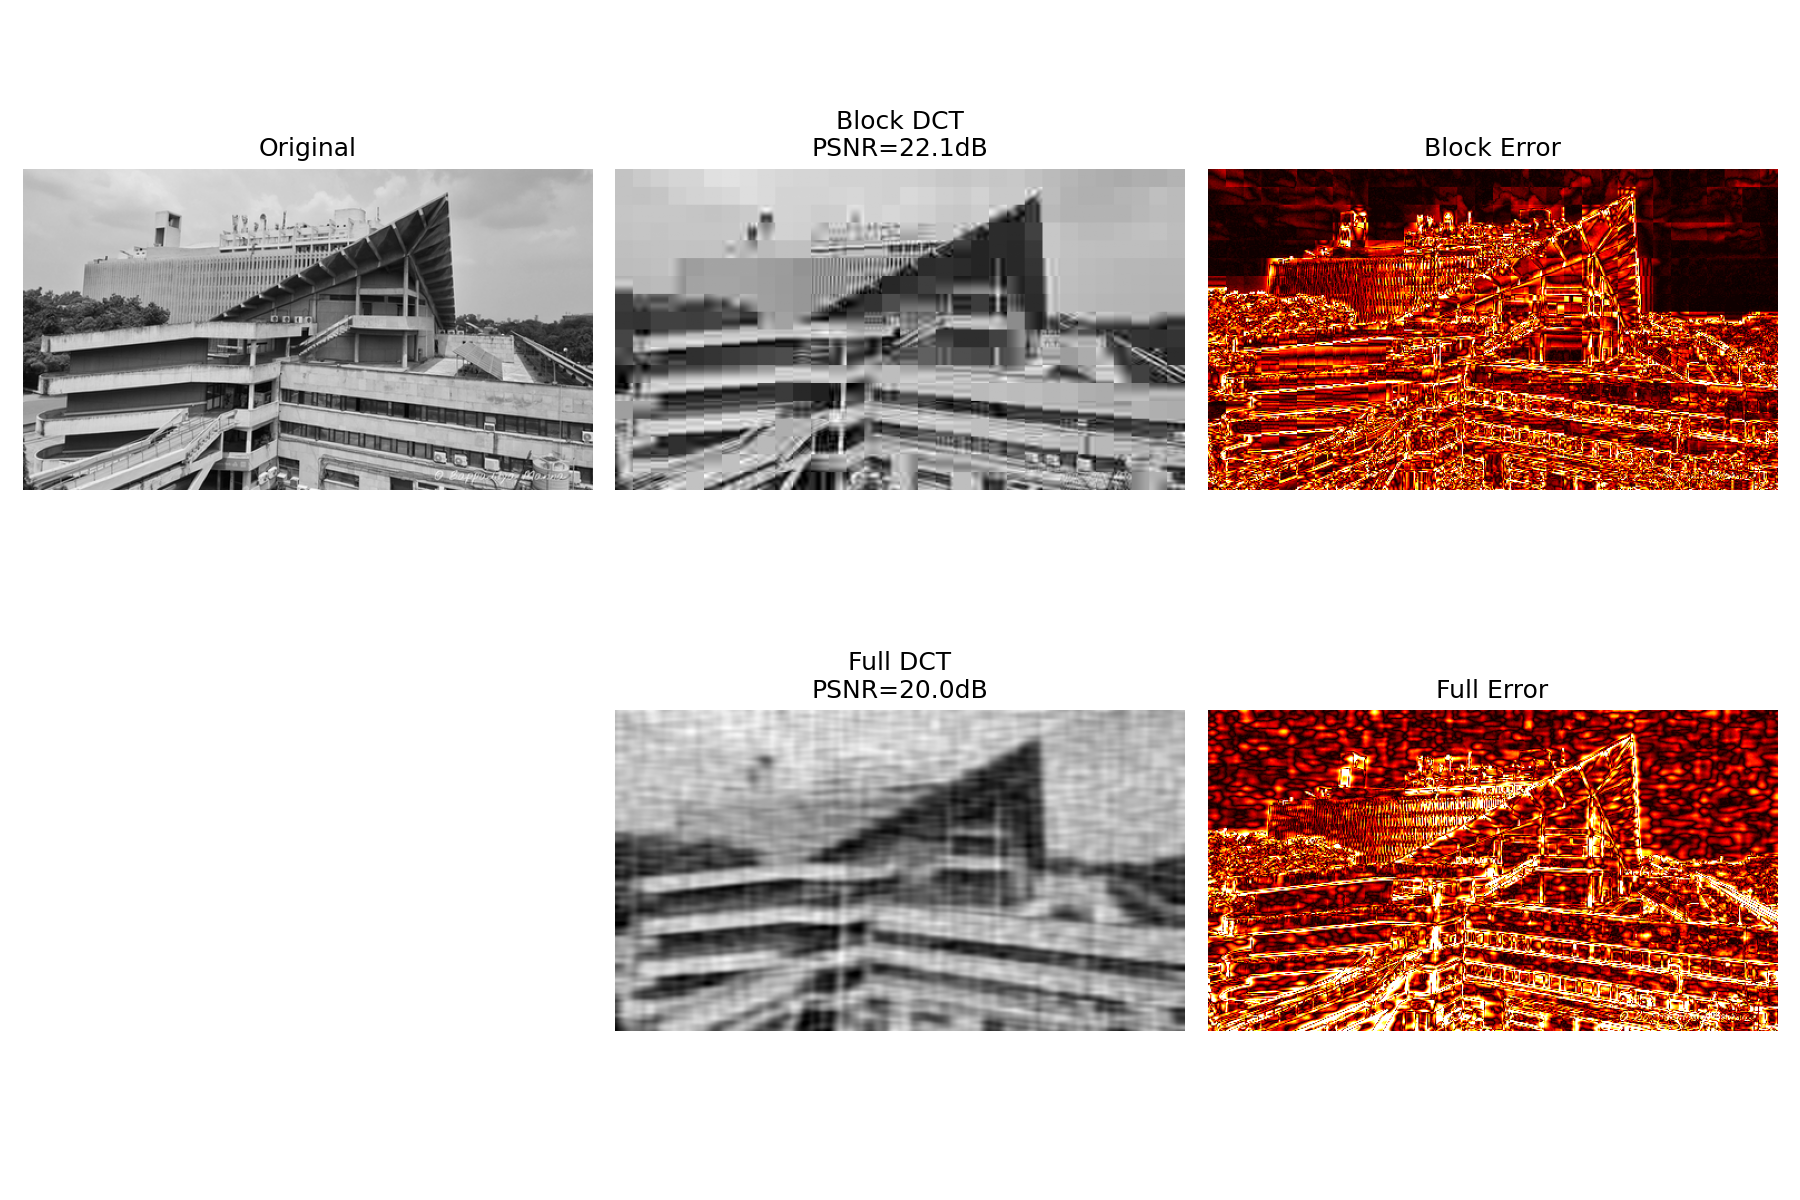
\includegraphics[width=0.95\textwidth]{part4/results/f2_comparison.png}
    \caption{Compression results for $f_2$ (photograph). Block DCT (top) vs. Full DCT (bottom).}
    \label{fig:f2_comp}
\end{figure}

\subsubsection{Discussion: Pros and Cons}
Based on the results, we can compare the two approaches:

\textbf{Block DCT (e.g., JPEG):}
\begin{itemize}
    \item \textbf{Pro:} Computationally efficient and memory-light. The transform is $O(N \log k)$ for $k=16$, which is much faster than the full transform's $O(N \log N)$ where $N=h \cdot w$.
    \item \textbf{Pro:} Locally adaptive. It can spend its "error budget" independently in each block. For image $f_1$, this was a huge advantage. It preserved the simple background blocks perfectly (zero error) and only introduced error in the complex blocks, leading to a high overall PSNR (26.9 dB).
    \item \textbf{Con:} Introduces blocking artifacts. The independent processing of blocks creates visible discontinuities at the $16 \times 16$ boundaries, which are visually jarring (see $f_2$ "Block DCT" image).
\end{itemize}

\textbf{Full DCT:}
\begin{itemize}
    \item \textbf{Pro:} Achieves optimal global energy compaction, as it considers all coefficients across the entire image.
    \item \textbf{Pro:} Does not produce blocking artifacts. The error is distributed more smoothly.
    \item \textbf{Con:} Computationally infeasible for large images. A $1024 \times 1024$ image would require a $1024^2 \times 1024^2$ transform, which is prohibitive.
    \item \textbf{Con:} Error is global. Dropping a single low-frequency coefficient introduces ringing artifacts or "ghosting" that spreads across the entire image (see $f_2$ "Full DCT" image).
    \item \textbf{Con:} Performs poorly on images with mixed content. For $f_1$, the error from the sharp lines was "smeared" across the entire image, polluting the previously perfect background areas. This forced the algorithm to drop to the minimum 20.0 dB PSNR, a much worse result than the block method.
\end{itemize}

\textbf{Conclusion:} The block-based DCT performs significantly better for the diagram image $f_1$ by localizing error. For the photographic image $f_2$, the block-based method also achieved a higher PSNR, and its main drawback (blocking artifacts) is often considered less objectionable than the global ringing artifacts of the full DCT. Given its massive computational advantage, the block-based approach is the clear practical winner.

\newpage
\section{Problem 5: PNG-like Compression with Predictive Coding, LZW, and Huffman}

\subsection*{Overview}
This problem implements a complete PNG-like image compression system that combines three complementary techniques:
\begin{enumerate}
    \item \textbf{Predictive coding} to reduce spatial redundancy
    \item \textbf{LZW compression} to exploit dictionary-based patterns
    \item \textbf{Huffman coding} to achieve entropy-optimal bit encoding
\end{enumerate}

The implementation works on \textbf{color (RGB) images}, processing all three channels throughout the pipeline. We test on the same two images from Problem 4: $f_1$ (diagram with flat regions) and $f_2$ (photographic image).

\subsection{Part (a): Predictive Coding with Paeth Predictor}
Following the PNG specification, we use the Paeth predictor for all interior pixels. For each pixel $(i,j)$, the prediction is based on three neighbors:
\begin{itemize}
    \item $a$: left pixel $(i, j-1)$
    \item $b$: upper pixel $(i-1, j)$
    \item $c$: upper-left pixel $(i-1, j-1)$
\end{itemize}

The Paeth predictor chooses the neighbor that is closest to $p = a + b - c$:
$$\text{Paeth}(a,b,c) = \begin{cases}
a & \text{if } |p-a| \leq |p-b| \text{ and } |p-a| \leq |p-c| \\
b & \text{if } |p-b| \leq |p-c| \\
c & \text{otherwise}
\end{cases}$$

For color images, this prediction is applied independently to each of the R, G, B channels. The prediction error is:
$$e_{i,j,c} = \text{pixel}_{i,j,c} - \text{prediction}_{i,j,c}$$

where $e \in [-255, 255]$ for each channel. Edge cases (top row, left column, top-left pixel) use simpler predictors.

\begin{figure}[H]
\centering
\begin{subfigure}[b]{0.45\textwidth}
    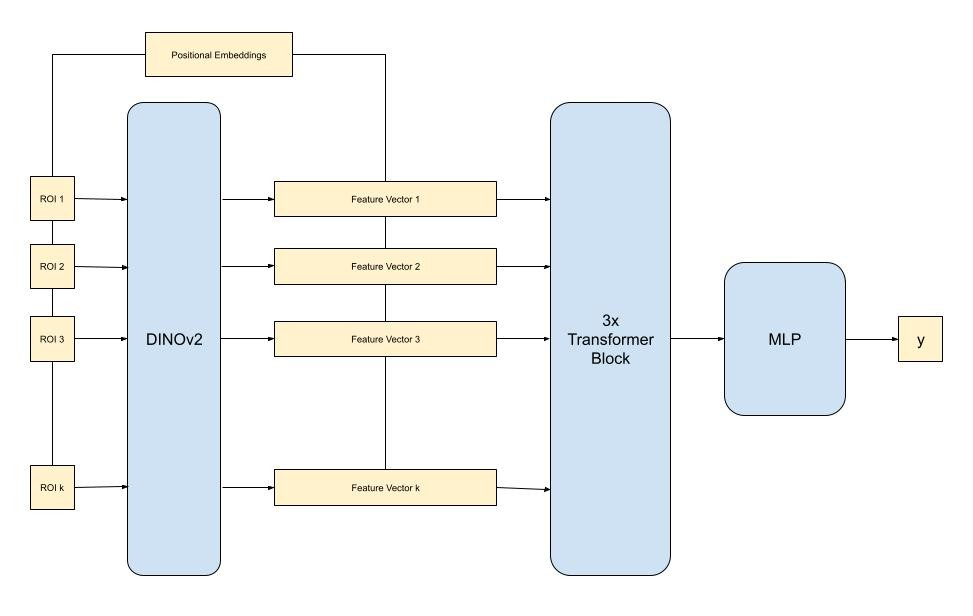
\includegraphics[width=\textwidth]{part5/results/f1_original.png}
    \caption{Original $f_1$ (diagram)}
\end{subfigure}
\hfill
\begin{subfigure}[b]{0.45\textwidth}
    
\includegraphics[width=\textwidth]{part5/results/f1_error.png}
    \caption{Prediction error $e_1$ (offset by 128)}
\end{subfigure}
\caption{Original image and prediction error for $f_1$}
\end{figure}

\begin{figure}[H]
\centering
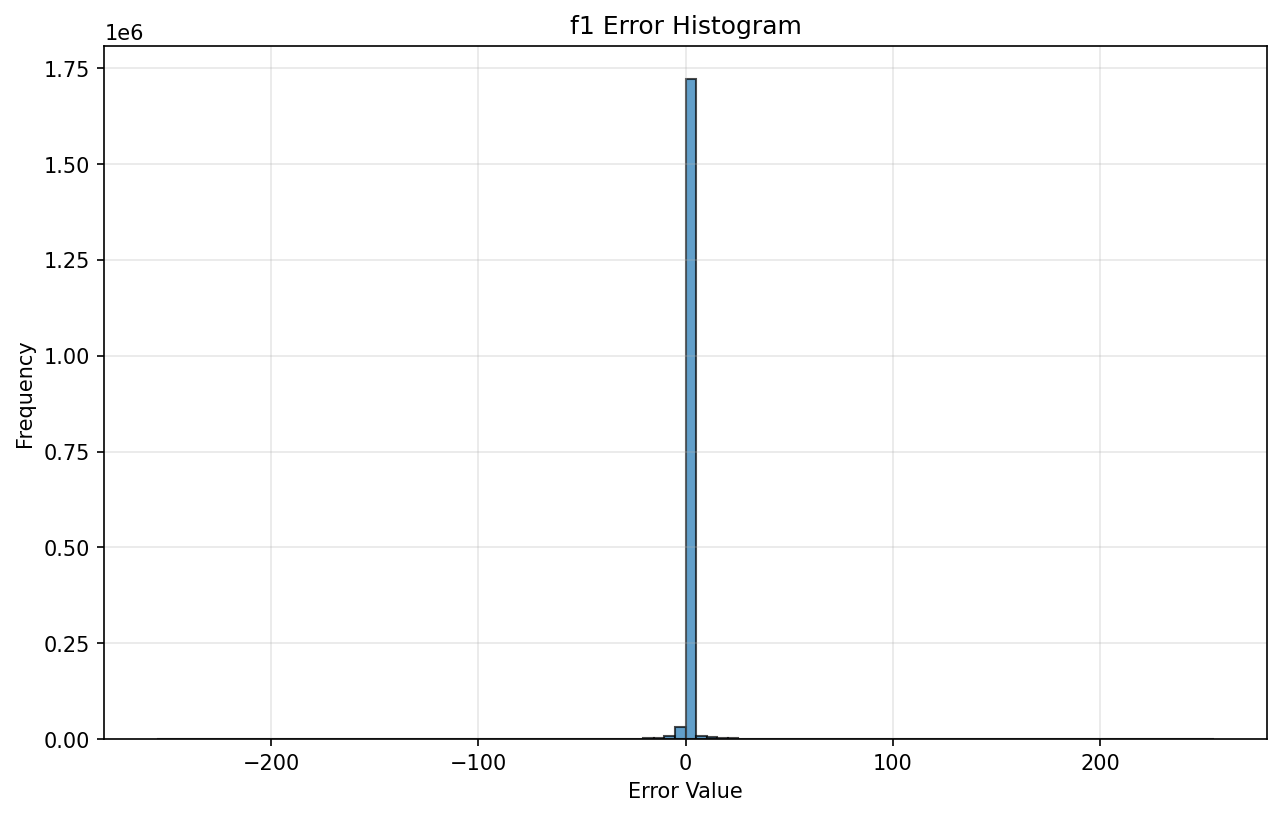
\includegraphics[width=0.8\textwidth]{part5/results/f1_hist.png}
\caption{Histogram of prediction errors for $f_1$ (all three color channels combined)}
\end{figure}

\textbf{Results for $f_1$ (diagram, $616 \times 973 \times 3$):}
\begin{itemize}
    \item Error standard deviation: $\sigma = 8.91$
    \item Error entropy: $H = 0.672$ bits/pixel
    \item Expected compression from prediction alone: $8/0.672 = 11.90\times$
\end{itemize}

The very low entropy (0.672 bits/pixel) indicates that the Paeth predictor is highly effective for this diagram image. Most prediction errors are concentrated near zero, as seen in the histogram.

\begin{figure}[H]
\centering
\begin{subfigure}[b]{0.45\textwidth}
    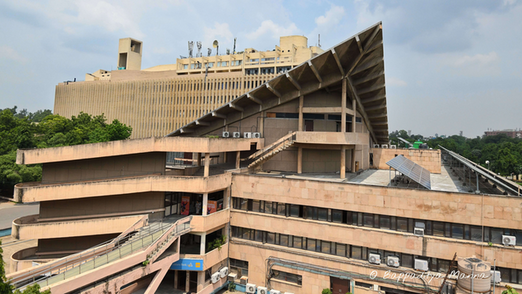
\includegraphics[width=\textwidth]{part5/results/f2_original.png}
    \caption{Original $f_2$ (photograph)}
\end{subfigure}
\hfill
\begin{subfigure}[b]{0.45\textwidth}
    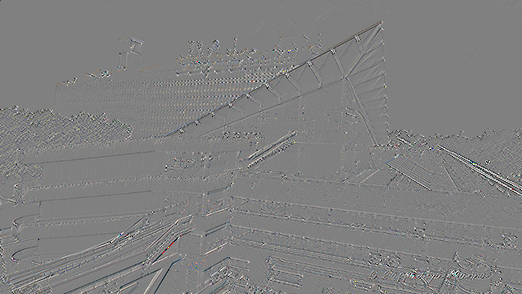
\includegraphics[width=\textwidth]{part5/results/f2_error.png}
    \caption{Prediction error $e_2$ (offset by 128)}
\end{subfigure}
\caption{Original image and prediction error for $f_2$}
\end{figure}

\textbf{Results for $f_2$ (photograph, $294 \times 522 \times 3$):}
\begin{itemize}
    \item Error standard deviation: $\sigma = 13.74$
    \item Error entropy: $H = 4.94$ bits/pixel
    \item Expected compression from prediction alone: $8/4.94 = 1.62\times$
\end{itemize}

The photographic image has much higher error entropy (4.94 bits/pixel) due to texture and detail that cannot be perfectly predicted from neighboring pixels.

\subsection{Part (b): Decoder Verification}
We implemented a decoder that reconstructs the original image from the error array by reversing the prediction process:
$$\text{pixel}_{i,j,c} = \text{clip}\left(\text{prediction}_{i,j,c} + e_{i,j,c}, 0, 255\right)$$

The decoder must apply predictions in the same scan order (left-to-right, top-to-bottom) to ensure each pixel's neighbors are already reconstructed when computing its prediction.

\begin{figure}[H]
\centering
\begin{subfigure}[b]{0.45\textwidth}
    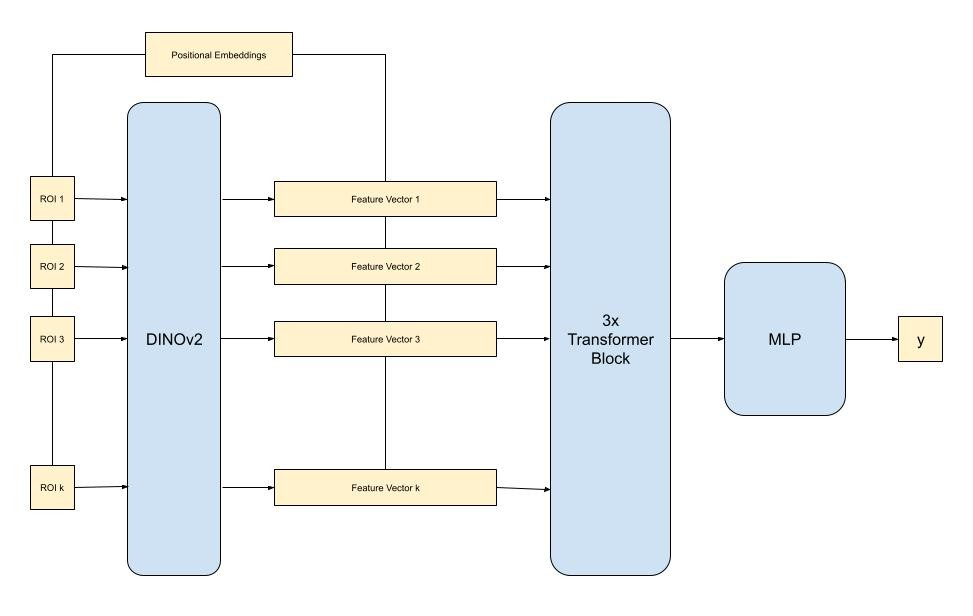
\includegraphics[width=\textwidth]{part5/results/f1_reconstructed.png}
    \caption{Reconstructed $f_1$}
\end{subfigure}
\hfill
\begin{subfigure}[b]{0.45\textwidth}
    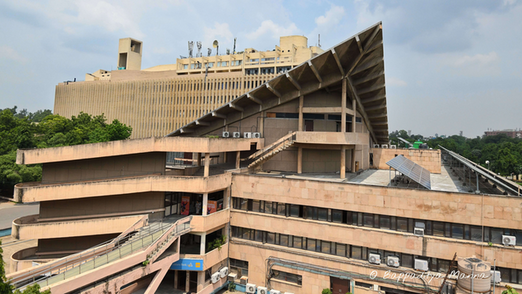
\includegraphics[width=\textwidth]{part5/results/f2_reconstructed.png}
    \caption{Reconstructed $f_2$}
\end{subfigure}
\caption{Perfect reconstruction from error images}
\end{figure}

\textbf{Verification results:}
\begin{itemize}
    \item $f_1$: Perfect reconstruction (\texttt{np.array\_equal} = True), max pixel difference = 0
    \item $f_2$: Perfect reconstruction (\texttt{np.array\_equal} = True), max pixel difference = 0
\end{itemize}

This confirms the prediction-recovery process is lossless and correctly implemented.

\subsection{Part (c): LZW Compression}

\subsubsection{Implementation Details}
The LZW encoder handles signed prediction errors in the range $[-255, 255]$:
\begin{enumerate}
    \item \textbf{Range mapping:} Errors are mapped to $[0, 511]$ by adding 255
    \item \textbf{Dictionary initialization:} 512 initial entries, each representing a single error value using 2-byte encoding
    \item \textbf{Corner case handling:} When the decoder encounters code $k$ that equals the current dictionary size, it correctly handles this by setting \texttt{entry = w + w[:2]}
\end{enumerate}

\subsubsection{Testing on Constant Sequences}
We tested LZW on sequences of $N$ zeros to verify the corner case and analyze complexity:

\begin{center}
\begin{tabular}{|c|c|c|}
\hline
\textbf{Input Length $N$} & \textbf{Output Length} & \textbf{$N/\text{len}^2$} \\
\hline
100 & 14 & 0.51 \\
1,000 & 45 & 0.49 \\
10,000 & 141 & 0.50 \\
100,000 & 447 & 0.50 \\
\hline
\end{tabular}
\end{center}

\textbf{Big-O Analysis:} For a constant sequence of length $N$, the LZW output length is $O(\sqrt{N})$.

\textbf{Proof:} The dictionary builds sequences $[0], [00], [000], \ldots$ After outputting $k$ codes, the total input consumed is:
$$1 + 2 + 3 + \cdots + k = \frac{k(k+1)}{2} \approx N$$

Solving for $k$: $k \approx \sqrt{2N}$, confirming $O(\sqrt{N})$ output length.

The empirical ratio $N/\text{len}^2 \approx 0.5$ matches the theoretical prediction of $\approx 2$.

\subsubsection{LZW on Prediction Errors}
After flattening the 3D error array (height $\times$ width $\times$ 3 channels), we apply LZW compression:

\textbf{Results for $f_1$:}
\begin{itemize}
    \item Input: 1,798,104 error values
    \item Output: 45,669 LZW codewords
    \item Compression ratio: $1,798,104 / 45,669 = 39.37\times$
    \item LZW roundtrip test: \textbf{OK} (perfect reconstruction)
\end{itemize}

\textbf{Results for $f_2$:}
\begin{itemize}
    \item Input: 460,404 error values
    \item Output: 146,930 LZW codewords
    \item Compression ratio: $460,404 / 146,930 = 3.13\times$
    \item LZW roundtrip test: \textbf{OK} (perfect reconstruction)
\end{itemize}

The dramatic difference in LZW compression reflects the different error patterns: $f_1$ has highly repetitive errors (many zeros), while $f_2$ has more varied errors.

\subsection{Part (d): Huffman Coding}
After LZW compression, the codewords are further compressed using Huffman coding:
\begin{enumerate}
    \item Compute frequency distribution of LZW codewords
    \item Build optimal prefix-free code tree using heap-based algorithm
    \item Encode codewords as variable-length bit sequences
\end{enumerate}

\textbf{Results for $f_1$:}
\begin{itemize}
    \item LZW codeword entropy: $H = 13.21$ bits/symbol
    \item Huffman average code length: $\bar{L} = 13.26$ bits/symbol
    \item Huffman efficiency: $H/\bar{L} = 0.9962$ (99.6\%)
    \item Total encoded bits: 605,732
\end{itemize}

\textbf{Results for $f_2$:}
\begin{itemize}
    \item LZW codeword entropy: $H = 13.99$ bits/symbol
    \item Huffman average code length: $\bar{L} = 14.02$ bits/symbol
    \item Huffman efficiency: $H/\bar{L} = 0.9980$ (99.8\%)
    \item Total encoded bits: 2,059,918
\end{itemize}

The Huffman coding achieves near-optimal compression (99.6-99.8\% efficiency), very close to the theoretical entropy limit.

\subsection{Part (e): Complete Pipeline and Compression Ratios}

\subsubsection{Full Encoder/Decoder Implementation}
The complete encoder combines all three stages:
\begin{verbatim}
encode_image(img):
    1. e = predict_row(img)           
    2. flat = flatten(e)               
    3. codes = lzw_encode(flat)        
    4. table = huffman_build(codes)    
    5. bits = huffman_encode(codes)    
    return (table, bits)
\end{verbatim}

The decoder reverses the process:
\begin{verbatim}
decode_image(shape, table, bits):
    1. codes = huffman_decode(bits, table)
    2. flat = lzw_decode(codes)
    3. e = reshape(flat, shape)
    4. img = recover_from_error(e)
    return img
\end{verbatim}

\subsubsection{Compression Performance}

\textbf{Image $f_1$ ($616 \times 973 \times 3 = 1,798,104$ bytes):}
\begin{itemize}
    \item Prediction stage: $8 / 0.672 = 11.90\times$ (expected)
    \item LZW stage: $39.37\times$
    \item Overall compression: $14,384,832 / 605,732 = \mathbf{23.75\times}$
    \item Final size: 75,716 bytes (from 1,798,104 bytes)
    \item Full pipeline reconstruction: \textbf{Perfect} (verified)
\end{itemize}

\textbf{Image $f_2$ ($294 \times 522 \times 3 = 460,404$ bytes):}
\begin{itemize}
    \item Prediction stage: $8 / 4.94 = 1.62\times$ (expected)
    \item LZW stage: $3.13\times$
    \item Overall compression: $3,683,232 / 2,059,918 = \mathbf{1.79\times}$
    \item Final size: 257,490 bytes (from 460,404 bytes)
    \item Full pipeline reconstruction: \textbf{Perfect} (verified)
\end{itemize}

The system achieves \textbf{lossless compression} with ratios ranging from 1.79$\times$ (complex photograph) to 23.75$\times$ (simple diagram). The compression ratio depends heavily on image content: diagrams with large flat regions compress extremely well, while photographs with texture compress modestly.

\subsection{Part (f): Optional Extensions}

\subsubsection{Per-Row Predictor Selection}
The standard PNG format allows choosing from 5 predictors per row:
\begin{enumerate}
    \item \textbf{None:} No prediction (use 0)
    \item \textbf{Left:} Use left neighbor $a$
    \item \textbf{Up:} Use upper neighbor $b$
    \item \textbf{Average:} Use $(a + b) / 2$
    \item \textbf{Paeth:} Use Paeth predictor
\end{enumerate}

For each row, we test all 5 predictors and choose the one with the lowest sum of squared errors. The predictor choice is stored (1 byte per row) and must be transmitted to the decoder.

\textbf{Results for $f_1$ with per-row selection:}
\begin{itemize}
    \item Per-row error entropy: 0.690 bits/pixel (vs. 0.672 baseline)
    \item Predictor usage: 55\% UP, 43\% PAETH, 1\% LEFT, 0.5\% AVG
    \item Per-row + LZW compression: $23.33\times$
    \item Observation: Slightly worse than fixed Paeth (23.75$\times$)
\end{itemize}

\textbf{Results for $f_2$ with per-row selection:}
\begin{itemize}
    \item Per-row error entropy: 4.941 bits/pixel (vs. 4.940 baseline)
    \item Predictor usage: 97\% PAETH, 1.4\% LEFT, 1\% AVG, 0.3\% UP
    \item Per-row + LZW compression: $1.79\times$
    \item Observation: Essentially identical to fixed Paeth
\end{itemize}

\textbf{Analysis:} For these images, per-row predictor selection does not improve compression. This is because:
\begin{itemize}
    \item Both images have consistent prediction characteristics across rows
    \item The overhead of storing predictor choices (1 byte per row) negates small gains
    \item Paeth predictor is already near-optimal for natural images
\end{itemize}

\subsubsection{Run-Length Encoding (RLE) Alternative}
We also implemented RLE as an alternative to LZW:
\begin{itemize}
    \item Each run is encoded as (value, count) pairs
    \item Maximum run length: 255
    \item These pairs are then Huffman-coded
\end{itemize}

\textbf{RLE Results:}
\begin{itemize}
    \item $f_1$ with RLE: $15.58\times$ (vs. $23.33\times$ with LZW)
    \item $f_2$ with RLE: $1.35\times$ (vs. $1.79\times$ with LZW)
\end{itemize}


\end{document}
